\documentclass[10pt,a4paper]{article}

\usepackage[T1]{fontenc}
\usepackage[utf8]{inputenc}
\usepackage[ngerman]{babel}
\usepackage{lmodern}
\usepackage{geometry}
\geometry{left=1.75cm,right=1.75cm,top=1.55cm,bottom=1.55cm}
\usepackage{setspace}
\setstretch{0.98}
\usepackage{enumitem}
\usepackage{graphicx}
\usepackage{hyperref}
\hypersetup{colorlinks=true,linkcolor=blue,urlcolor=blue}
\setlist[itemize]{leftmargin=1.1em,itemsep=0.05em,topsep=0.05em,parsep=0pt,partopsep=0pt}
\pagestyle{empty}

\begin{document}

\begin{center}
{\Large \textbf{Triagent: One-Pager für potenzielle Design-Partner}}\\[0.15em]
{\large AI-unterstützte, on-prem-fähige Phishing-Triage für Security-Teams}\\[0.35em]
\textbf{Alexander Hülsmann und Tassilo Bechtolsheim} -- Produkt- und Prototyp-Stand April 2026
\end{center}
\small

\vspace{0.25em}
\noindent\textbf{Worum es bei Triagent grundsätzlich geht}\\
Triagent ist ein \textbf{Workspace für die Bearbeitung gemeldeter verdächtiger E-Mails}. Die Grundidee ist nicht, einen Analysten durch eine Black-Box-Klassifikation zu ersetzen. Die Grundidee ist, \textbf{manuelle Triage-Arbeit zu verkürzen}: gemeldete E-Mails schneller vorsortieren, technische Evidenz automatisch zusammenführen, einen ersten Entscheidungsentwurf liefern und daraus einen \textbf{nachvollziehbaren, exportierbaren Fall} machen.

\vspace{0.25em}
\noindent\textbf{Die größere Vision}\\
Kurzfristig startet Triagent bei \textbf{reported-email triage}: also bei genau dem Moment, in dem Mitarbeiter oder Systeme verdächtige Mails melden und ein Analyst entscheiden muss, ob es sich um Phishing, Business Email Compromise, Malware, Spam oder einen harmlosen Fall handelt.\\
Mittelfristig soll daraus ein \textbf{lokal betreibbarer Evidence-Layer für E-Mail-Incidents} werden:
\begin{itemize}
  \item automatische Trennung zwischen \textbf{analystenwürdigen Fällen} und \textbf{Low-Value-Meldungen},
  \item konsistente Evidenzsammlung über Header, Auth, URLs, Anhänge und Message Source hinweg,
  \item AI-unterstützte Entwürfe für Klassifikation und Fallabschluss,
  \item später auch \textbf{kampagnenweises Arbeiten} statt mehrfacher Einzelfallprüfung ähnlicher Mails.
\end{itemize}

\noindent\textbf{Welches Problem adressiert wird}
\begin{itemize}
  \item Reported Phishing ist in vielen Teams weiterhin \textbf{stark manuell}.
  \item Analysten springen zwischen Mail-Client, Header-/Auth-Checks, URL-Tools, Sandbox, Tickets und Dokumentation.
  \item Viel Aufwand steckt nicht nur in der Analyse, sondern in \textbf{Begründung, Auditierbarkeit und Export}.
  \item In regulierten oder sensiblen Umfeldern sind \textbf{Cloud-only-Workflows} oft organisatorisch oder datenschutzseitig schwierig.
\end{itemize}

\noindent\textbf{Was im aktuellen Prototyp bereits funktioniert}
\begin{itemize}
  \item \textbf{Intake und Meldung:} Upload von \texttt{.eml} und \texttt{.msg} sowie Outlook-Add-in für das Melden aus dem Client.
  \item \textbf{Analysten-Workspace:} getrennte Sichten für \texttt{Uploads} als Intake-/Fallliste und \texttt{In-tray} als priorisierte Analysten-Queue.
  \item \textbf{Automatische Vorsortierung:} frühe Triage-Buckets wie \texttt{Needs investigation}, \texttt{Likely benign} und \texttt{Uncertain}. Dieser Teil ist \textbf{noch in einem sehr frühen Stadium} und muss vor produktivem Einsatz noch deutlich weiter getuned und validiert werden.
  \item \textbf{Technische Analyse:} SPF, DKIM, DMARC, ARC, Reply-To- und Return-Path-Signale, URL-Extraktion mit Redirect-Auflösung, Attachment-Metadaten, X-Headers, Transmission Hops und Raw Source.
  \item \textbf{AI-unterstützte Resolution:} früher Assist-Draft mit vorgeschlagener Disposition, Klassifikationscode und markierten Artefakten, immer analyst-in-the-loop. Auch dieser Teil ist aktuell \textbf{Demo- und Prototyp-Logik}, nicht schon produktionsreif.
  \item \textbf{Evidenz und Exporte:} PDF-, Markdown- und JSON-Export für Fallberichte sowie IOC-Export als JSON oder CSV.
  \item \textbf{Governance:} Audit Log, Rollen- und Rechtekonzept, API Keys und reproduzierbare Demo-Datensätze.
\end{itemize}

\noindent\textbf{Was noch fehlt oder bewusst noch nicht als fertig gilt}
\begin{itemize}
  \item \textbf{Kein produktionsreifes Enterprise-Produkt}: der aktuelle Stand ist ein starker Demo- und Pilot-Prototyp.
  \item \textbf{Tiefe Integrationen} in Ticketing, SIEM, SOAR oder bestehende Mail-Security-Plattformen sind noch nicht fertig ausgebaut.
  \item \textbf{Enterprise SSO / IdP} und weitergehende Betriebs- und Packaging-Themen sind noch offen.
  \item \textbf{Kampagnen-Handling} ist im Backend angelegt, aber noch nicht der klar validierte Primär-Workflow.
  \item \textbf{Messbarer Kundennutzen} wie Zeitersparnis, Auto-Close-Raten oder Zahlungsbereitschaft muss noch in echten Pilot-Setups validiert werden.
\end{itemize}

\noindent\textbf{Tech-Stack des Prototyps}
\begin{itemize}
  \item \textbf{Frontend:} Next.js, React, TypeScript
  \item \textbf{Backend:} FastAPI, Python
  \item \textbf{Datenhaltung:} PostgreSQL
  \item \textbf{ORM / Migrationen:} SQLAlchemy, Alembic
  \item \textbf{Artefakte / Storage:} MinIO als S3-kompatibler Objektspeicher
  \item \textbf{Deployment:} heute Docker Compose und self-hosted; perspektivisch sowohl \textbf{on-prem} als auch \textbf{Cloud} verfügbar
  \item \textbf{Client-Integration:} Outlook Add-in auf Basis von Office.js
\end{itemize}

\noindent\textbf{Warum das für Design-Partner interessant sein kann}
\begin{itemize}
  \item Sie können früh beeinflussen, \textbf{welcher reale Triage-Workflow} zuerst sauber gelöst wird.
  \item Sie helfen zu validieren, \textbf{wo die größte Hebelwirkung liegt}: automatische Vorsortierung, schnellere Evidenzsammlung, sauberere Fallabschlüsse oder kampagnenweises Arbeiten.
  \item Sie bekommen früh Einblick in ein Tool, das \textbf{lokal betreibbar}, analystenorientiert und auf nachweisbare Entscheidungen ausgelegt ist.
\end{itemize}

\noindent\textbf{Wonach aktuell gesucht wird}
\begin{itemize}
  \item Security-Teams, SOCs oder MSSPs mit wiederkehrendem reported-email-Volumen
  \item 30- bis 45-minütige Workflow-Gespräche oder ein gemeinsamer Blick auf synthetische / anonymisierte Beispielcases
  \item perspektivisch 1 bis 3 Design-Partner, um einen klar abgegrenzten Pilot-Workflow zu testen
\end{itemize}

\noindent\textbf{Kurz gesagt}\\
Triagent ist heute \textbf{kein weiteres generisches ``AI Security Tool''}, sondern ein konkreter Prototyp für \textbf{AI-unterstützte, evidence-first Phishing-Triage}. Der Kernwert liegt darin, Analysten \textbf{nicht jeden gemeldeten Fall gleich behandeln zu lassen}, sondern Low-Value-Meldungen von analystenwürdigen Fällen zu trennen und für die wichtigen Fälle schnell eine nachvollziehbare Entscheidungsgrundlage zu liefern.

\newpage

\begin{center}
{\Large \textbf{Produkt-Eindrücke aus dem aktuellen Prototyp}}\\[0.25em]
\small Reale Screenshots aus dem aktuellen Demo-Stack
\end{center}

\vspace{0.35em}
\noindent\textbf{1. Resolution-Flow mit Assist-Draft und analyst-in-the-loop-Freigabe}\\[0.2em]
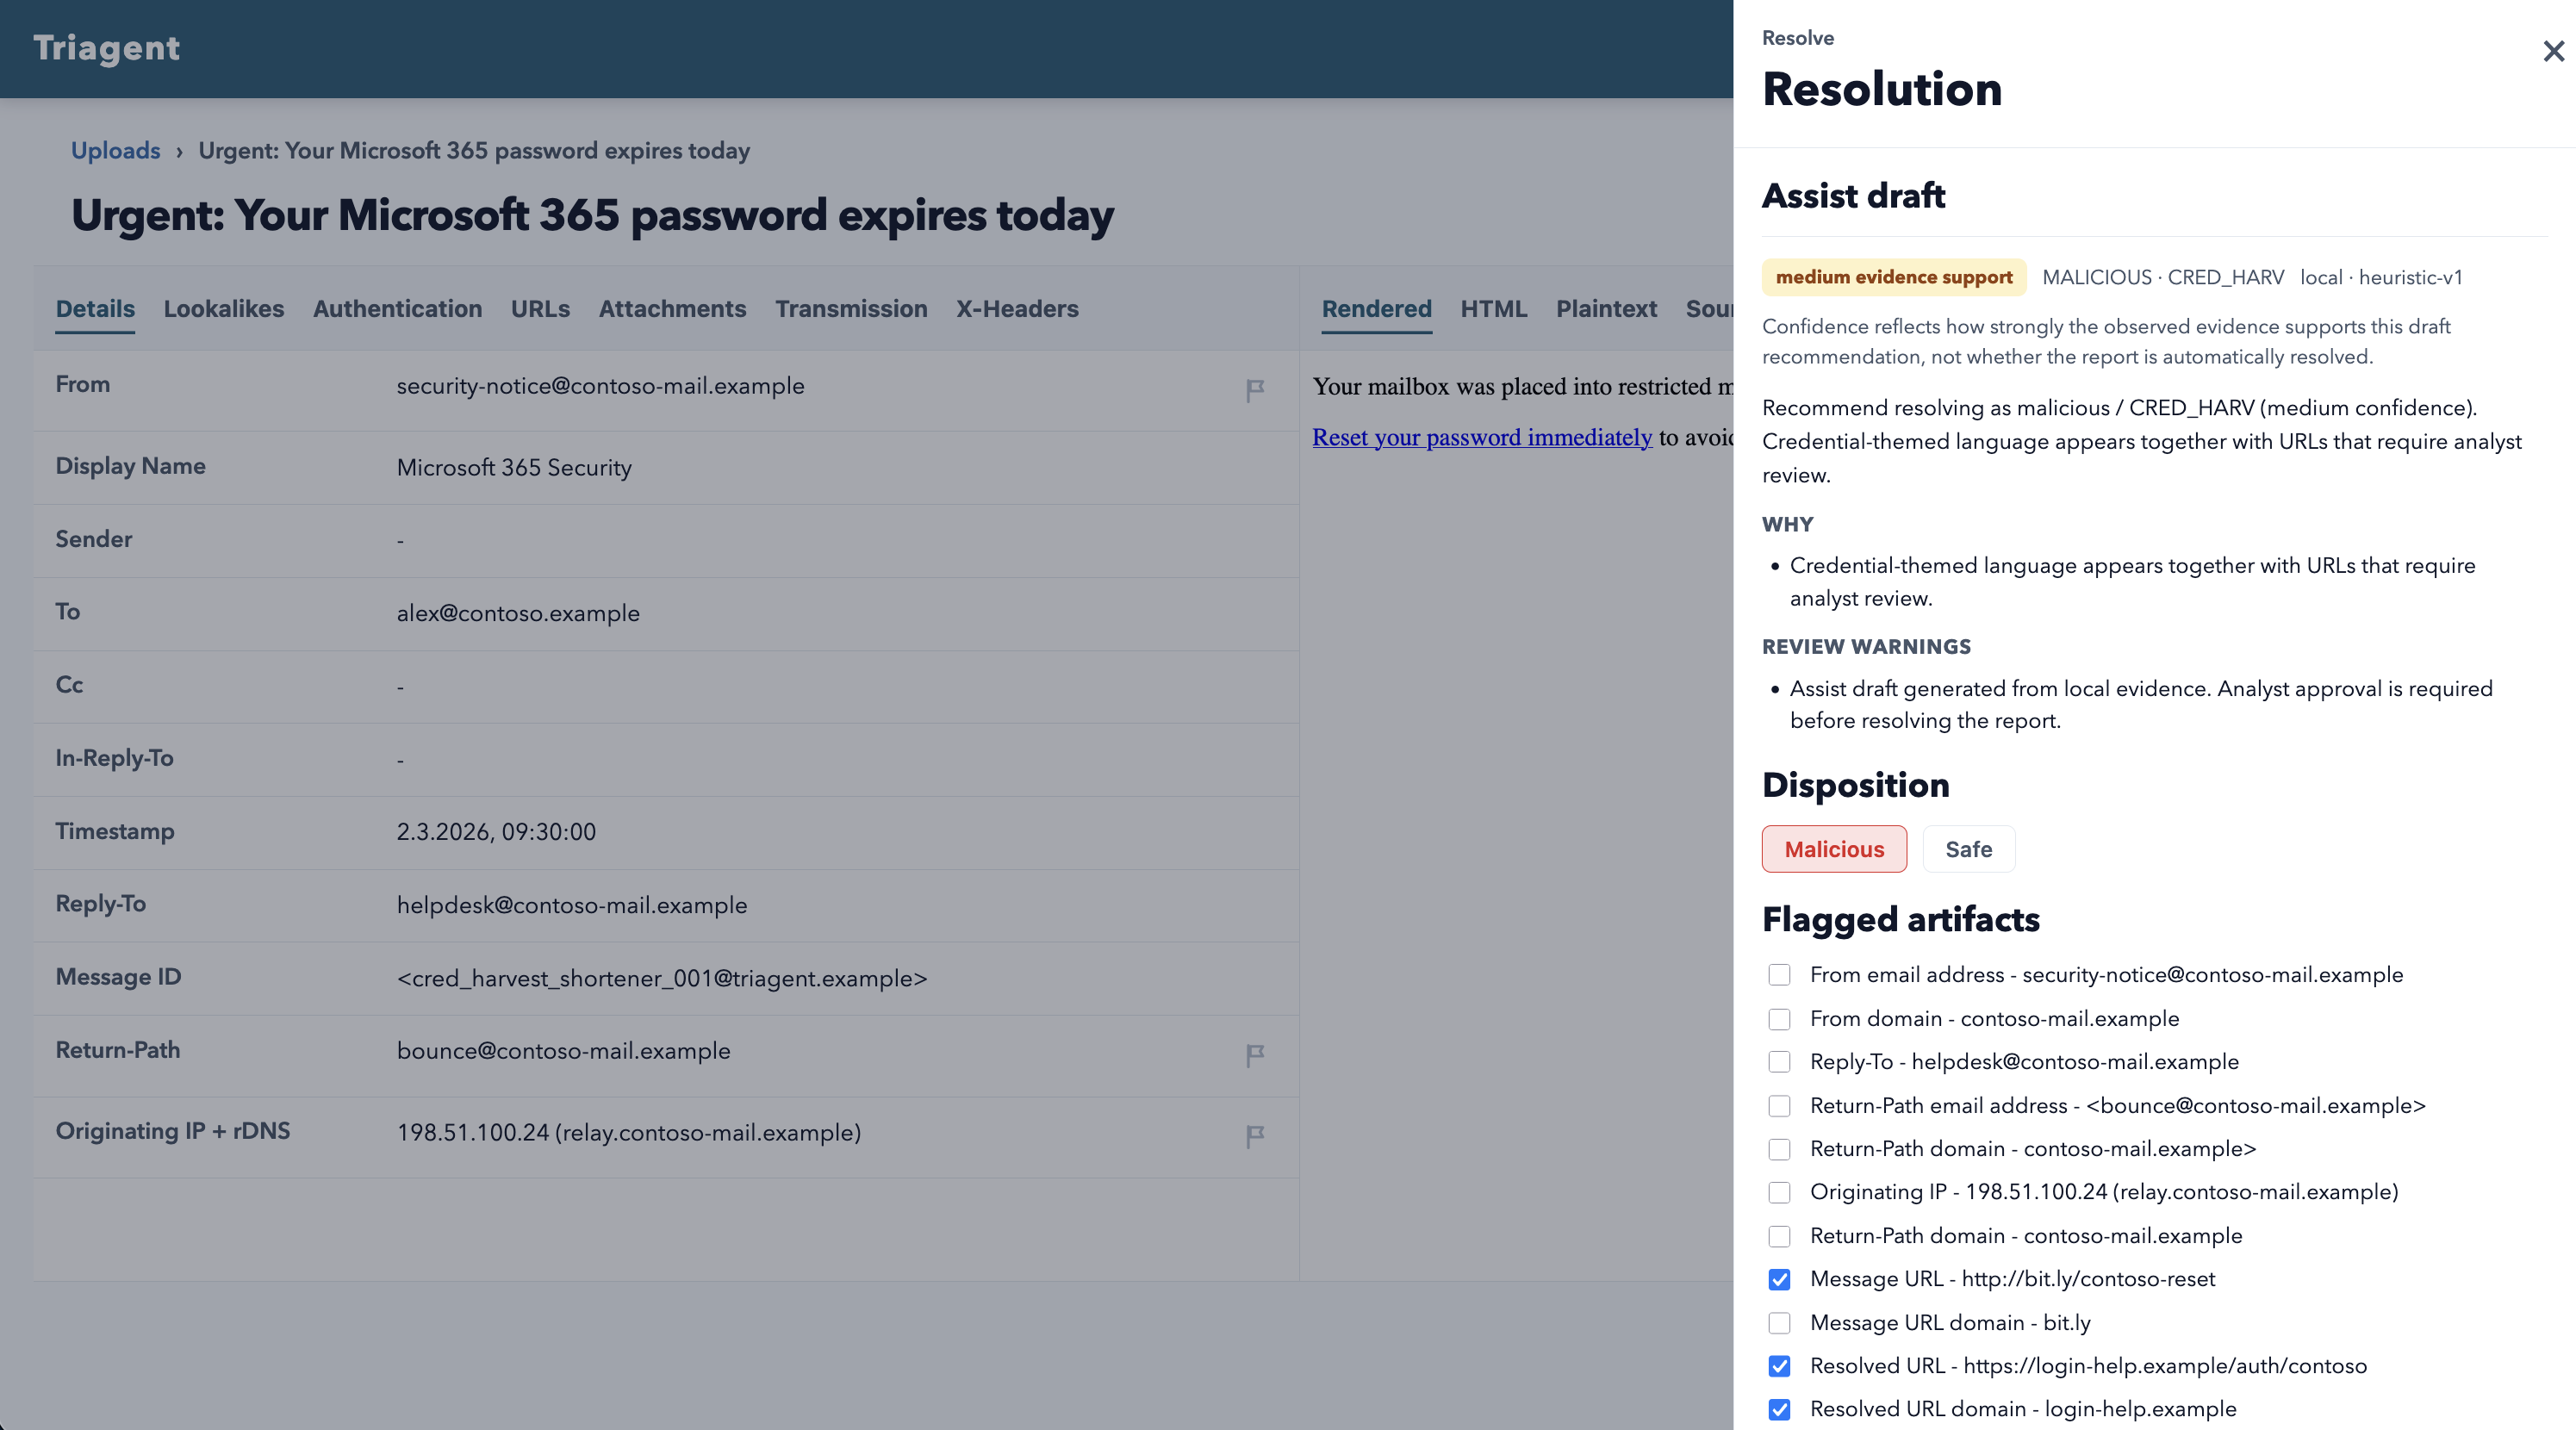
\includegraphics[width=\textwidth]{../../ResolutionFlow.png}

\vspace{0.45em}
\noindent\textbf{2. Analysten-Queue / Uploads}\\[0.2em]
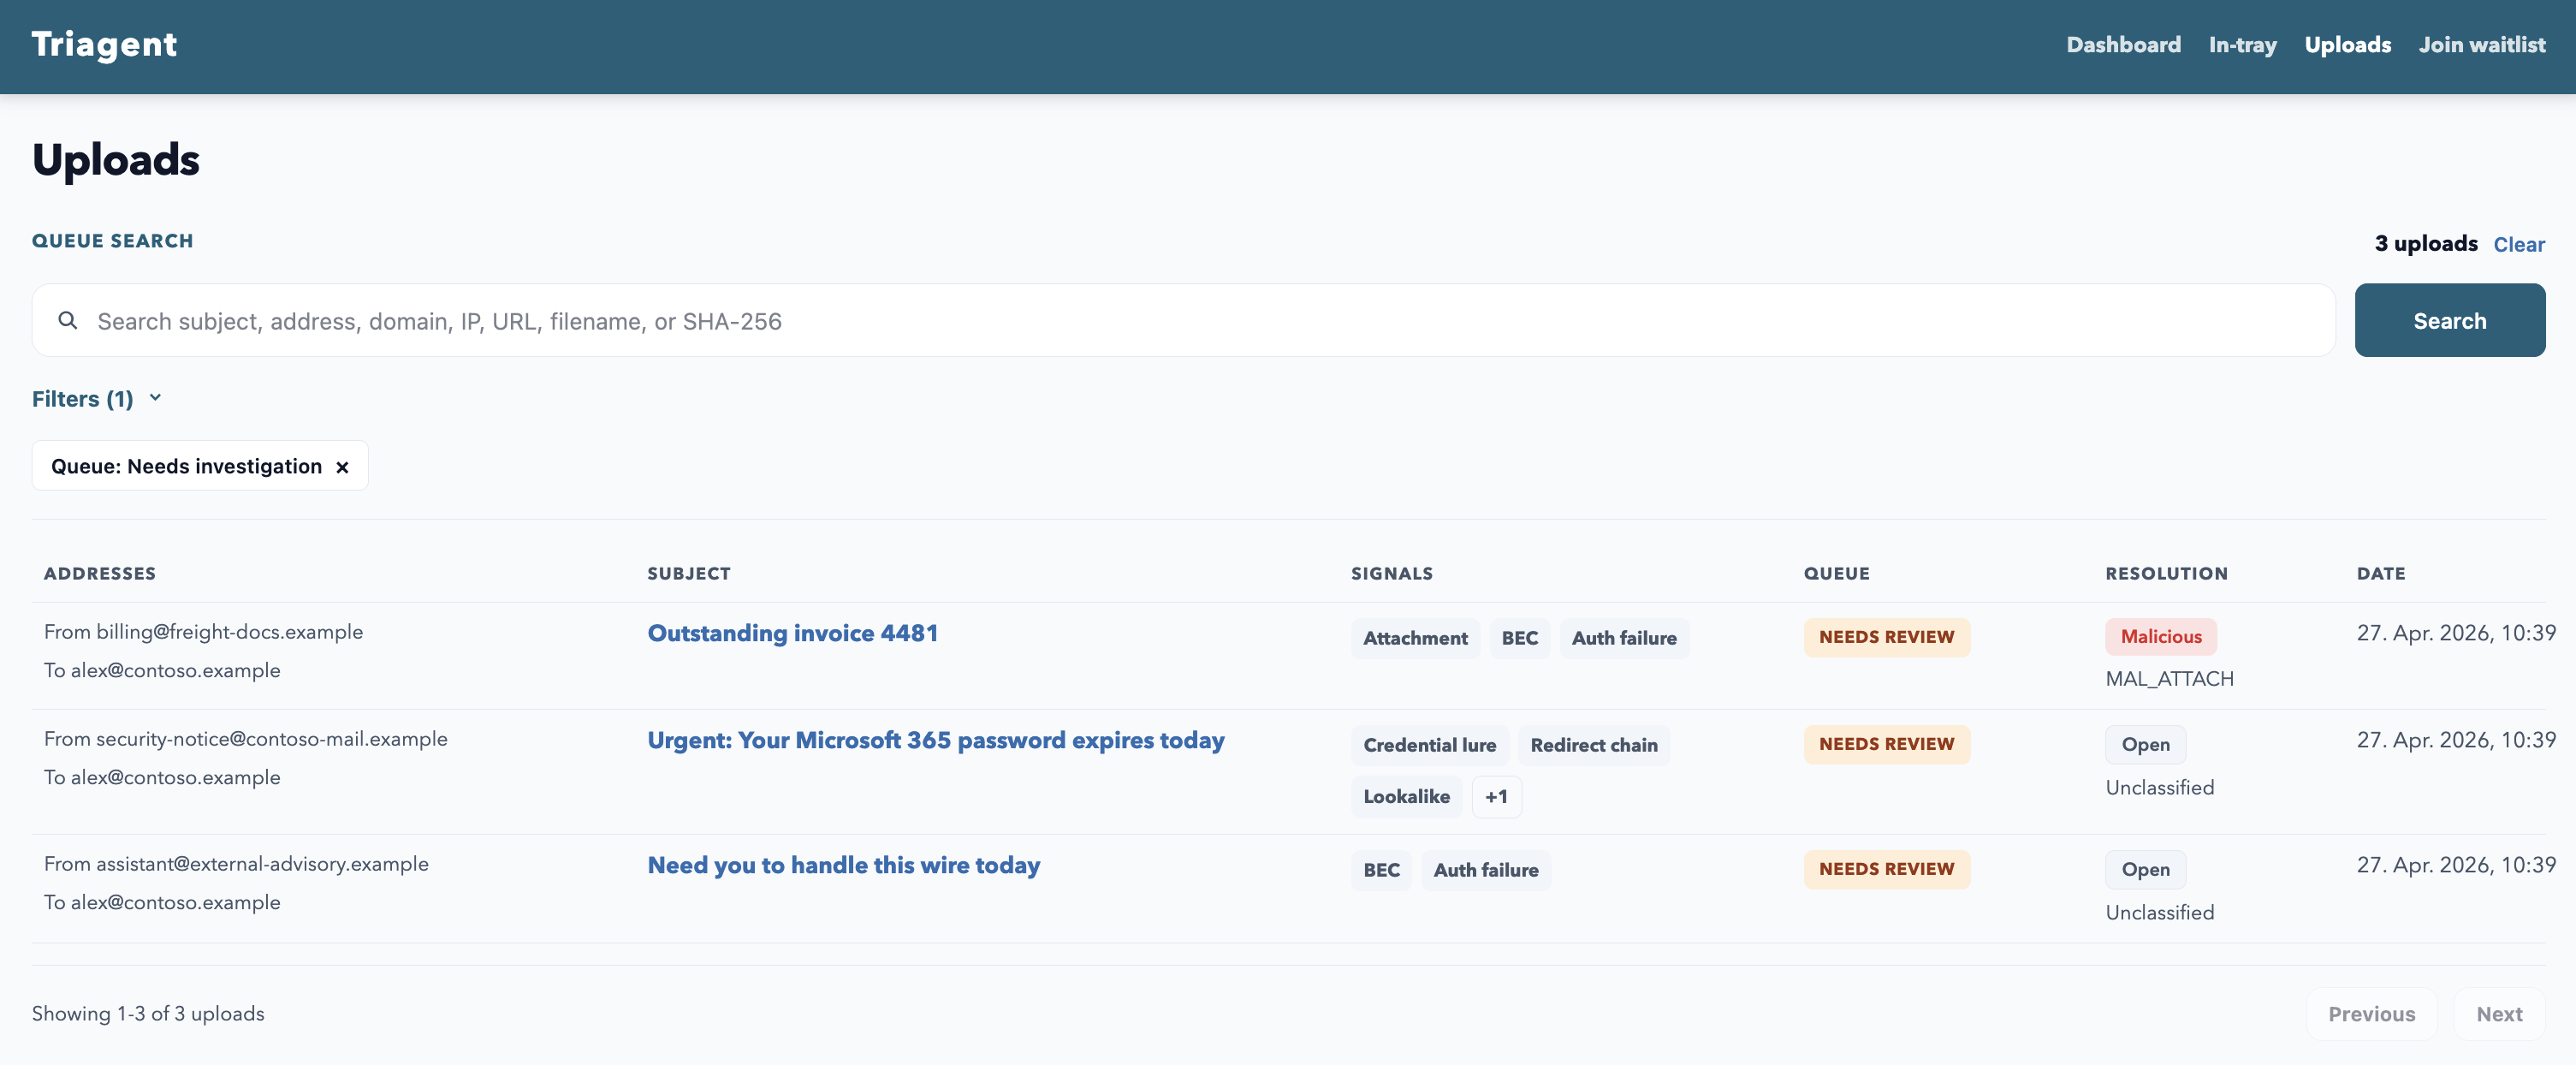
\includegraphics[width=\textwidth]{../../Queue.png}

\vspace{0.45em}
\noindent\textbf{3. Dashboard / Überblick}\\[0.2em]
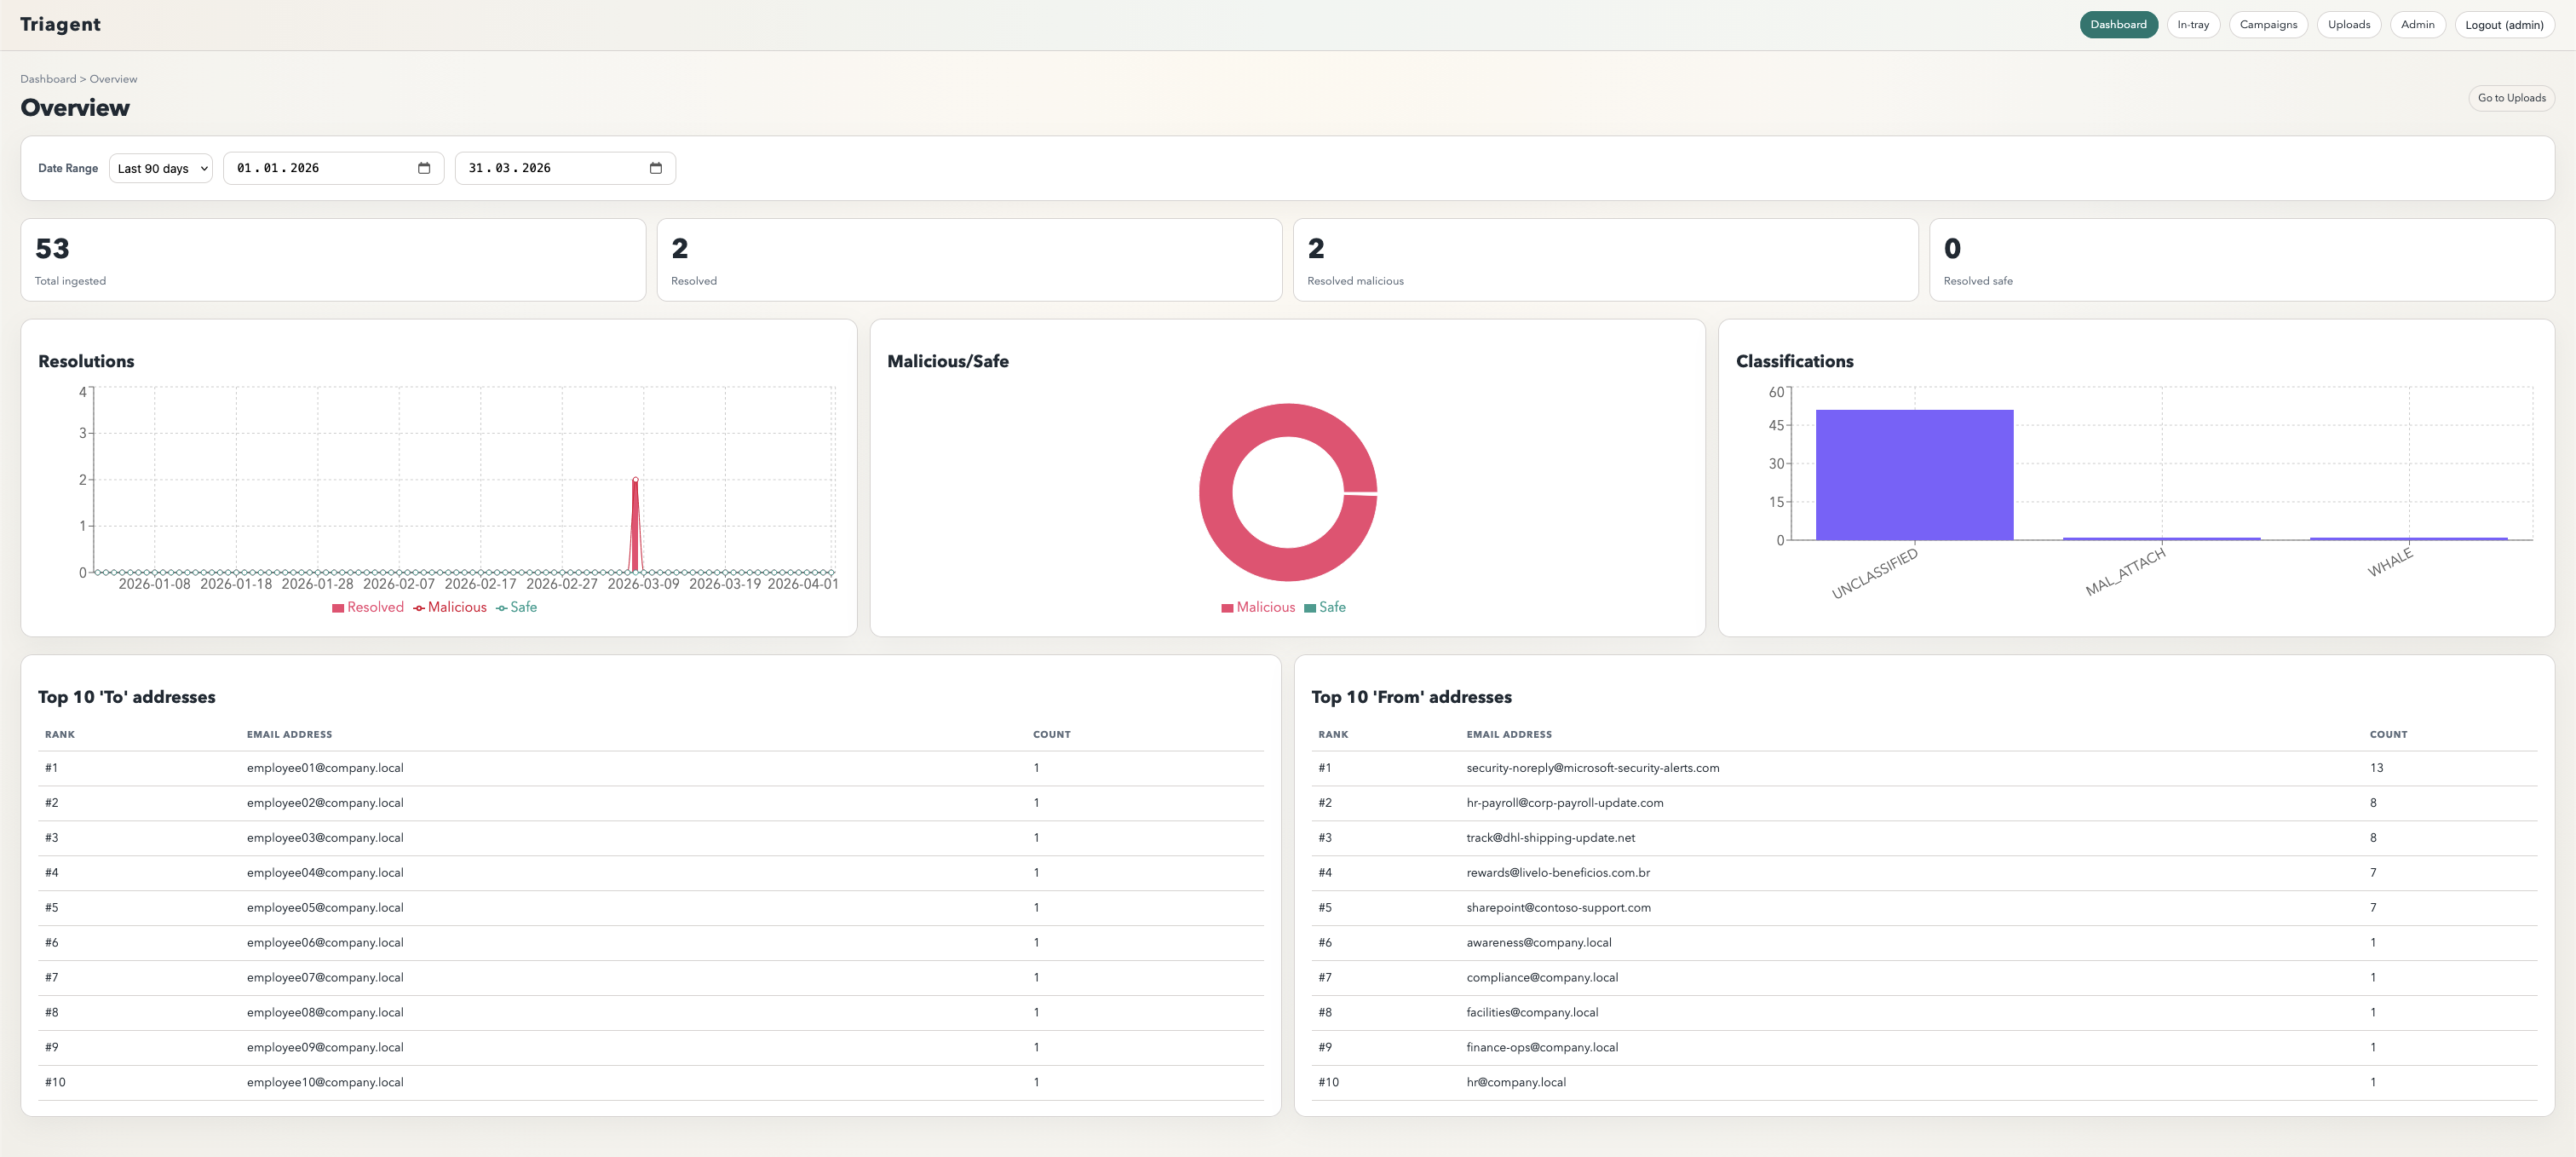
\includegraphics[width=\textwidth]{../../Dashboard.png}

\end{document}
